\chapter{Decadimenti Nucleari}
\section{Decadimento}
Molti elementi in natura sono caratterizzati da atomi non stabili.

Di solito una sostanza radioattiva decade in un'altra, anch'essa radioattiva.
In questo caso si dice che le due sostanze sono in \textit{relazione genetica}
(sostanza madre e sostanza figlia).
Quando si hanno catene di sostanze radioattive si parla di \textit{famiglie}.

Consideriamo una miscela di due sostanze in relazione genetica (1=madre, 
2=figlia).
Siano $N_1(0)$ e $N_2(0)$ i numeri di atomi a $t=0$. Ci si chiede quali siano i
valori $N_1(t)$ e $N_2(t)$.

Sappiamo che per la sostanza 1 vale la legge
\begin{equation}
dN_1=-N_1(t)\lambda_1dt.
\end{equation}
Ciascun atomo che decade si trasforma nella sostanza 2.
Quindi le variazioni della sostanza 2 sono dovute a due effetti opposti:
\begin{equation}
\label{diff_n2}
dN_2=\lambda_1 N_1(t)dt-\lambda_2 N_2(t)dt.
\end{equation}

Supponiamo che sia $\lambda_1\neq\lambda_2$. Per trovare le funzioni $N_1(t)$ e 
$N_2(t)$
procediamo per tentativi considerando le due funzioni
\begin{equation}
\label{func_dec}
N_1(t)=A_{11}e^{-\lambda_1t}\qquad 
N_2(t)=A_{21}e^{-\lambda_1t}+A_{22}e^{-\lambda_2t}
\end{equation}
Per le condizioni iniziali deve essere:
\[
N_1(0)=A_{11}\qquad N_2(0)=A_{21}+A_{22}
\]

Per determinare $A_{21}$ e $A_{22}$ sostituiamo le due funzioni \eqref{func_dec}
nell'equazione differenziale per $N_2$ (\eqref{diff_n2}). Si ottiene che:
\begin{align*}
&dN_2=\lambda_1A_{11}e^{-\lambda_1t}dt-\lambda_2[A_{21}e^{-\lambda_1t}+A_{22}e^{
-\lambda_2t}]dt=\\
&=[(\lambda_1A_{11}-\lambda_2A_{21})e^{-\lambda_1t}-\lambda_2A_{22}e^{-\lambda_2
t}]dt
\end{align*}
Questo deve essere eguagliato all'espressione:
\[
dN_2=[-\lambda_1A_{21}e^{-\lambda_1t}-\lambda_2A_{22}e^{-\lambda_2t}]dt
\]
$N_2$ è soluzione se e solo se:
\[
-\lambda_1A_{21}=\lambda_1A_{11}-\lambda_2A_{21}\Rightarrow 
A_{21}=A_{11}\frac{\lambda_1}{\lambda_2-\lambda_1}
\]

Quindi\marginnote{11-2-1998} le due espressioni per $N_1$ e $N_2$ in questo 
caso sono:
\begin{gather}
N_1(t)=N_1(0)e^{-\lambda_1t}\\
N_2(t)=N_1(0)\frac{\lambda_1}{\lambda_2-\lambda_1}e^{-\lambda_1t}+[N_2(0)-N_1(0)
\frac{\lambda_1}{\lambda_2-\lambda_1}]e^{-\lambda_2t}
\end{gather}
\section{Decadimento Duale}
Consideriamo ora il caso in cui una sostanza madre ha più sostanze figlie.
In questo caso si ha cioè più di un canale di decadimento e ciascun canale 
sarà caratterizzato da un particolare meccanismo dinamico,
che per lo più si identifica con l'emissione $\alpha$ o $\beta$.

In questo caso si parla di \textit{decadimento duale} o \textit{diramazione}.
Consideriamo per esempio un atomo caratterizzato da un decadimento duale con 
emissioni $\alpha$ e $\beta$;
siano $\lambda_{\alpha}$ e $\lambda_{\beta}$ le corrispondenti costanti di 
disintegrazione.
Le equazioni che regolano questi due processi sono:
\begin{gather}
-dN_{\alpha}(t)=N(t)\lambda_{\alpha}dt\footnotemark\\
-dN_{\beta}(t)=N(t)\lambda_{\beta}dt\footnotemark
\end{gather}

\addtocounter{footnote}{-1}
\footnotetext{Numero di atomi che si disintegrano nell'intervallo di tempo d$t$
per emissione $\alpha$}
\stepcounter{footnote}
\footnotetext{Numero di atomi che si disintegrano nell'intervallo di tempo d$t$
per emissione $\beta$}

Il numero totale di atomi che si disintegrano risulta dunque:
\begin{equation}
-dN(t)=-dN_{\alpha}(t)-dN_{\beta}(t)=N(t)[\lambda_{\alpha}+\lambda_{\beta}]dt
\end{equation}

Quindi $\lambda_{\alpha}+\lambda_{\beta}$ è la costante di disintegrazione 
totale. Si definiscono i \textit{rapporti di diramazione}:
\begin{gather}
R_{\alpha}=\frac{dN_{\alpha}(t)}{dN(t)}=\frac{\lambda_{\alpha}}{\lambda_{\alpha}
+\lambda_{\beta}}\\
R_{\beta}=\frac{dN_{\beta}(t)}{dN(t)}=\frac{\lambda_{\beta}}{\lambda_{\alpha}+\l
ambda_{\beta}}
\end{gather}
$R_{\alpha}$ dà la percentuale di decadimento $\alpha$, $R_{\beta}$ la 
probabilità di decadimento $\beta$.

Se escludiamo la fissione spontanea, che comunque è un processo abbastanza 
raro, i decadimenti radioattivi naturali sono essenzialmente tre:
$\alpha$,$\beta$,$\gamma$. Questi tre tipi di decadimento si identificano in 
realtà con ben determinate trasformazioni spontanee dei nuclei atomici.

\section{Decadimento $\alpha$}

Quando un atomo emette una particella $\alpha$ il nucleo subisce la
trasformazione:
\begin{equation}
\mathcal{N}(A,Z)\rightarrow\mathcal{N}(A-4,Z-2)+\alpha.
\end{equation}

La condizione che dev'essere verificata affinché questo decadimento possa
avvenire spontaneamente è che la massa iniziale del nucleo deve risultare
maggiore della somma delle masse delle particelli finali. Questa condizione
corrisponde ad una diminuzione dell'energia del sistema, infatti se ci si pone
in un sistema di riferimento in cui il nucleo iniziale è a riposo, il
decadimento può avvenire solo se viene liberata una certa energia cinetica,
cioè:
\begin{equation}
E_d=M(A,Z)c^2-[M(A-4,Z-2)+m_{\alpha}]c^2>0;
\end{equation}
questa quantità  si dice \textit{energia di decadimento}. Se si utilizza la
formula semiempirica delle masse nucleari, considerato che la massa della
particella $\alpha$ è 
$m_{\alpha}\simeq\frac{3728}{c^2}\si{\mega\electronvolt}$,
si trova che l'energia di decadimento $E_d$ risulta positiva solo se $A<150$.
Questa previsione risulta in perfetto accordo con i dati sperimentali. Si deve
anche notare che la relativa facilità con cui un decadimento $\alpha$ avviene 
è
dovuta al fatto che la particella $\alpha$ ha un difetto di massa piuttosto
grande ($\simeq28,3/c^2\,\si{\mega\electronvolt}$); questo fatto favorisce il
decadimento $\alpha$ da un punto di vista energetico.

Sperimentalmente si trova che l'energia cinetica $T_{\alpha}$ con cui viene
emessa la particella $\alpha$ assume valori all'interno dell'intervallo
$4\,\si{\mega\electronvolt}\lesssim T_{\alpha}\lesssim
9\,\si{\mega\electronvolt}$.

Questo implica che:
\[
\frac{T_{\alpha}}{m_{\alpha}c^2}<\frac{1}{800}=1,25\permil
\]
e quindi è una buona approssimazione considerare il moto della particella
$\alpha$ nel limite non relativistico:
\[
T_{\alpha}=\frac{p^2}{2m_{\alpha}}
\]
\begin{equation}
  \begin{split}
  E_d&=\frac{p^2}{2m_{\alpha}}+\frac{p^2}{2M(A-4,Z-2)}=\\
  
&=\frac{p^2}{2}\frac{m_{\alpha}+M(A-4,Z-2)}{m_{\alpha}M(A-4,Z-2)}=T_{\alpha}\fra
c{m_{\alpha}+M(A-4,Z-2)}{M(A-4,Z-2)}
\end{split}
\end{equation}
Per nuclei sufficientemente pesanti si può trascurare l'energia cinetica del
nucleo prodotto dal decadimento.

In contrasto con la modesta variabilità di $T_{\alpha}$ si riscontra
sperimentalmente una grande varietà di tempi di vita media. Questi tempi 
infatti
variano da un ordine di grandezza minimo di $10^{-7}\si{\second}$($Po^{212}$,
polonio), fino a un ordine di grandezza massimo di $10^{10}$ anni ($Th^{232}$,
torio). Il primo caso corrisponde al valore massimo di $T_{\alpha}\simeq
9\,\si{\mega\electronvolt}$, mentre il secondo corrisponde al valore minimo,
$T_{\alpha}\simeq 4\,\si{\mega\electronvolt}$. Nella maggioranza dei casi il
tempo di vita media risulta comunque di qualche secondo.

\breaknote

Abbiamo\marginnote{25-2-1998} visto che i due casi estremi per il tempo di vita
media e per l'energia della particella $\alpha$ sono:
\begin{align*}
&Po^{212}\quad\tau_{\alpha}\simeq 10^{-7}\,\si{\second}\quad T_{\alpha}\simeq 
9\,\si{\mega\electronvolt}\\
&Th^{232}\quad\tau_{\alpha}\simeq 10^{10}\,anni\quad T_{\alpha}\simeq 
4\,\si{\mega\electronvolt}
\end{align*}

Nella maggior parte dei casi si ha $\tau_{\alpha}\simeq 1\,\si{\second}$. Se si
cerca di trattare il decadimento $\alpha$ in termini classici si giunge ad un
paradosso. Consideriamo il nucleo $\mathcal{N}(A,Z)$ come se fosse virtualmente
composto da un altro nucleo e da una particella $\alpha$, cioè:
\[
\mathcal{N}(A,Z)=\mathcal{N}(A',Z')+\alpha\qquad A'=A-4,Z'=Z-2
\]
Consideriamo l'andamento dell'energia potenziale $V(r)$ della particella
$\alpha$, dove $r$ è la distanza dal nucleo. Se $R'$ è il raggio del nucleo
virtuale si ha che:
\[
V(r)=\frac{2Z'e^2}{r}\quad r>R'
\]
Per $r<R'$ si sentono pure le forze nucleari. Per descrivere questo caso
possiamo considerare una buca rettangolare di profondità fissata. In questa
ipotesi l'andamento di $V(r)$ è (\autoref{fig:pot_nucl_p97}):

\begin{figure}[hbtp]
\centering
\caption{Potenziale nucleare.}
\label{fig:pot_nucl_p97}
\begin{tikzpicture}[line cap=round,line join=round,>=stealth ,x=1.0cm,y=1.0cm]
  \draw[->,color=black] (-0.37,0) -- (8.05,0);
  \foreach \x in {,0.5,1,1.5,2,2.5,3,3.5,4,4.5,5,5.5,6,6.5,7,7.5,8}
  \draw[shift={(\x,0)},color=black] (0pt,2pt) -- (0pt,-2pt);
  \draw[->,color=black] (0,-0.62) -- (0,2.72);
  \foreach \y in {-0.5,0.5,1,1.5,2,2.5}
  \draw[shift={(0,\y)},color=black] (2pt,0pt) -- (-2pt,0pt);
  \draw[smooth,samples=100,domain=2.5:8.05120201415096] plot(\x,{1/((\x)-2)});
  \draw [dash pattern=on 1pt off 1pt] (2.5,2)-- (2.5,0);
  \draw [dash pattern=on 1pt off 1pt] (2.5,2)-- (0,2);
	\fill [color=\MainColor] (2.5,0) circle (1.5pt);
	\draw[color=\MainColor] (2.56,0.09) node [anchor=north] {$R'$};
	\fill [color=\MainColor] (0,2) circle (1.5pt);
	\draw[color=\MainColor] (0.1,2.09) node [anchor=east] {$V_M$};
\end{tikzpicture}

\end{figure}

Possiamo supporre nota l'energia totale della particella $\alpha$ (a grandi
distanze l'energia totale si ridurrà a quella cinetica che può essere 
misurata).
Possiamo quindi porre:
\[
E=T_{\alpha}=\frac{1}{2}mv_{\alpha}^2
\]
Per la particella $\alpha$ è lecito trascurare l'energia a riposo. In termini
classici si trova che il tempo di permanenza della particella $\alpha$ nel
nucleo o è molto più breve di quello che è, oppure è infinito, questo a 
secondo
se può essere superata o meno la barriera di potenziale. Se la barriera è
sufficientemente bassa, l'emissione dovrebbe avvenire in un tempo:
\begin{equation}
\tau^{l}<\tau_0=\frac{2R'}{v_{\alpha}}=2R'\sqrt{\frac{m_{\alpha}}{2T_{\alpha}}}<
10^{-21}\,\si{\second}
\end{equation}
questo perchè $v_{\alpha}$ è minore della velocità della particella 
all'interno
della buca. Quando l'energia non è tale da poter superare la barriera, allora
classicamente l'emissione non può mai avvenire, cioè $\tau^{l}=\infty$. Questo
paradosso può essere risolto con l'uso della meccanica quantistica ed in
particolare grazie all'effetto tunnel. Cioè se la particella ha una energia
$E=T_{\alpha}<V_{max}$ vi è una probabilità non nulla che la particella superi
la barriera. Sia $\Delta t$ l'intervallo di tempo che la particella $\alpha$
impiegherebbe mediamente a superare la barriera. Per il principio di Heisenberg
deve essere:
\[
\Delta E=\frac{\hbar}{\Delta t}\Rightarrow E=T_{\alpha}\pm\frac{\Delta E}{2}
\]
anche se vale sempre $\mean{E}=T_{\alpha}$. Quindi l'attraversamento è 
possibile se
$\frac{\Delta E}{2}$ risulta:
\[
\frac{\Delta E}{2}\gtrsim V_{max}-T_{\alpha}
\]
Il processo che porta la particella $\alpha$ al di là della barriera di
potenziale viola il principio di conservazione dell'energia. Questo però è un
processo virtuale, e non misurabile o osservabile. La grandezza che caratterizza
questo processo è il \textit{coefficiente di trasmissione} ($C_T$). Questo dà 
la
possibilità che un singolo urto contro la barriera faccia uscire la particella
$\alpha$. Affinché il decadimento possa avvenire la particella $\alpha$ deve
urtare in media $\frac{1}{C_T}$ volte. Quindi l'effettivo tempo di vita media 
è:
\[
\tau=\frac{1}{C_T}\tau_0\qquad C_T<<1;
\]
da questo si deduce che $C_T$ deve essere la causa del fatto che
sperimentalmente $\tau>>\tau_0$. Affrontiamo il problema in modo più rigoroso:
se lo spin del nucleo
iniziale è nullo si trova che:
\[
C_T=e^{-2G}
\]
dove
\begin{equation}
G=G(T_{\alpha},Z',R')\simeq\frac{2e^2Z'}{\hbar}\sqrt{\frac{2m_{\alpha}}{T_{\alph
a}}}
= \frac{4}{\hslash}\sqrt{m_\alpha Z'R'}
\end{equation}
in questo caso si deduce che
\[
\tau=\tau_0e^{2G}
\]
La quantità $e^{2G}$ si dice \textit{fattore di Gamow} (questa è la teoria di 
Gamow per il decadimento $\alpha$). La dipendenza logaritmica di $\tau$ da 
$T_{\alpha}$
riproduce abbastanza bene i risultati sperimentali. Per esmpio possiamo 
considerare uno dei casi estremi, cioè il decadimento di $U^{238}$ nel 
$Th^{234}$, cioè
\[
  \text{U}^{238}\rightarrow \text{Th}^{234}+\alpha
\]
$T_{\alpha}\simeq 4,2\,\si{\mega\electronvolt}$, $Z'=90$, $R'=1,2\cdot 
234^{1/3}\cdot 10^{-13}\,\si{\centi\meter}\simeq 7,4\cdot 
10^{-13}\,\si{\centi\meter}$.
Sostituendo questi dati si trova il risultato
\[
2G\simeq173-83=90\Rightarrow C_T=e^{-90}\simeq10^{-39}
\]
Se immaginiamo il nucleo di $U^{238}$ virtualmente composto dal nucleo di 
$Th^{234}$ e dalla particella $\alpha$, si ha che la probabilità che la 
particella $\alpha$
quando urta sulla barriera del nucleo del $Th^{234}$ la superi, è pari a 
$10^{-39}$. Da questi si deduce che il tempo di vita media è:
\[
\tau_0=C_T\tau\simeq2\cdot10^{-22}\,\si{\second}
\]
dove $\tau\simeq2\cdot10^{17}\,\si{\second}$. Quindi il modello risulta 
coerente.

Il decadimento $\alpha$ avviene in generale fra stati fondamentali dei nuclei.
Esistono però casi in cui il nucleo finale possa trovarsi in uno o più stati
finali.
A questi casi corrisponde uno spettro a righe per la particella $\alpha$.
Supponiamo che il nucleo finale possa trovarsi o nello stato fondamentale $E_0$,
o negli stati eccitati
$E_1$ e $E_2$. In questo caso i valori per l'energia cinetica $T_{\alpha}^{(i)}$
sono:
\begin{align*}
&T_{\alpha}^{(0)}=T_{\alpha}\\
&T_{\alpha}^{(1)}=T_{\alpha}-(E_1-E_0)\\
&T_{\alpha}^{(2)}=T_{\alpha}-(E_2-E_0)
\end{align*}
Decadimenti $\alpha$ di questo tipo hanno una stretta connessione con le
radioattività naturali di raggi $\gamma$, in quanto un nucleo in uno stato
eccitato
decade subito nello stato fondamentale con l'emissione di uno o più fotoni
$\gamma$ (decadimento a cascata). L'energia dei fotoni $\gamma$ è\footnote{Su
questo valore non si è sicuri, nel testo originale è incomprensibile, pag. 
100}
:
\[
E_{\gamma}=cp_{\gamma}\simeq10^{-1}\,\si{\mega\electronvolt}
\]
La corrispondente energia cinetica di rinculo del nucleo è:
\[
 
T_R=\frac{1}{2}\frac{p_R}{M}=\frac{1}{2}\frac{p_{\gamma}}{M}=\frac{1}{2}\frac{E_
{\gamma}}{Mc^2}\simeq0,5\frac{10^{-2}}{10^5}\si{\mega\electronvolt}=5\cdot10^{-8
}\si{\mega\electronvolt}
\]
dove $M$ è la massa del nucleo finale, $p_R$  la quantità di moto del nucleo,
$p_{\gamma}$ la quantità di moto del fotone. Per il conto si è posto 
$M\simeq100$
\footnote{Si suppone siano 100 UM anche se nel testo originale non c'è
scritto.}.
Quindi un nucleo che emette un fotone $\gamma$ emetterà un energia di 
decadimento:
\[
E_d=E_{\gamma}+T_R\simeq E_{\gamma}
\]
quindi l'intera energia di decadimento viene trasportata dal fotone, si ha che:
\[
E_{\gamma}\simeq E_i-E_f
\]
dove $E_i$ e $E_f$ sono l'energia iniziale e finale del nucleo.
\section{Decadimento $\beta$}
Esistono\marginnote{27-2-1998} due tipi di emissioni spontanee di tipo $\beta$, 
queste si dicono $\beta^-$ e $\beta^+$.
Nel primo caso si ha che:
\begin{align*}
&\beta^-\quad \mathcal{N}(A,Z)\rightarrow\mathcal{N}(A,Z+1)+e^-+\bar{\nu}\quad 
n\rightarrow p^+\\
&\beta^+\quad \mathcal{N}(A,Z)\rightarrow\mathcal{N}(A,Z-1)+e^++\nu\quad 
p^+\rightarrow n
\end{align*}
transizioni di questo genere possono avvenire solo fra nuclei isobari.
Dal punto di vista energetico questi decadimenti risultano possibili solo se 
sono soddisfatte le condizioni:
\[
E_d^{\beta^{\pm}}=M(A,Z)c^2-[M(A,Z\pm1)+m_e+m_{\nu}]c^2>0
\]
dove si considera a riposo il nucleo iniziale. Normalmente si assume 
$m_{\nu}=0$, in quanto sperimentalmente si è trovato che:
\[
m_{\nu}<\frac{60}{c^2}\si{\electronvolt}<<m_e=\frac{0,5}{c^2}\si{\mega\electronv
olt}
\]
Il decadimento $\beta^+$ equivale alla trasformazione di un protone in un 
neutrone, il decadimento $\beta^-$ alla trasformazione inversa.
Il processo:
\[
n\rightarrow p^++e^-+\bar{\nu}
\]
avviene spontaneamente anche per un neutrone libero in quanto:
\[
m_n-m_p\simeq1,29\frac{\si{\mega\electronvolt}}{c^2}
\]
Il processo inverso
\[
p^+\rightarrow n+e^++\nu
\]
può verificarsi spontaneamente solo all'interno di un nucleo in quanto 
$m_p<m_n$, e non in un protone libero. A questo riguardo ci si può chiedere
come mai esistano nuclei isobari per cui:
\[
M(A,Z)>M(A,Z-1)
\]
La risposta a questo viene dalla formula  per le masse nucleari ed il fatto è 
che la presenza di un neutrone può fare diminuire l'energia elettrostatica di 
più di
quanto cambierebbe l'energia a riposo se invece si avesse un protone. 
L'elettrone e il positrone emessi in questi decadimenti mostrano uno spettro 
continuo di energia,
al contrario di quanto avviene nei decadimenti $\alpha$ e $\gamma$. Se si ha un 
insieme statistico si trova che le energie variano in maniera continua fra un 
valore minimo
ed uno massimo. Questo fu uno dei fatti che portò all'introduzione del 
neutrino. La natura continua di questi spettri presenta una difficoltà di 
principio in quanto
questi decadimenti corrispondono al passaggio fra due stati ben definiti del 
nucleo, si ha che l'elettrone e il positrone hanno un'energia che non
corrisponde a quella del passaggio di stato del nucleo tranne quando 
l'elettrone e il positrone hanno energia massima.
Quindi apparentemente manca una parte di energia. L'introduzione del neutrino 
serve quindi a mantenere valido il principio di conservazione dell'energia.
Un altro fatto che suggeriva la presenza del neutrino era pure l'apparente 
violazione della conservazione del momento angolare.

Per vedere questo consideriamo ad esempio il decadimento del trizio, la cui 
reazione è:
\[
H^3\rightarrow He^3+e^-
\]
Lo spin iniziale è $\frac{1}{2}$ mentre lo spin finale è o $0$ o $1$. Il 
momento angolare totale iniziale è semintero, mentre quello finale è 
sicuramente intero.
Se si vuole mantenere il principio di conservazione del momento angolare si 
deve introdurre una particella che deve per forza avere spin $1/2$.
Quindi il decadimento è:
\[
H^3\rightarrow He^3+e^-+\nu
\]
Quindi si introducono due nuove particelle, neutrino e antineutrino, queste 
erano considerate differenti per assunzione, ma per simmetria si ipotizzò
che fossero una particella e un antiparticella.

Un'altra emissone spontanea di un neutrino si ha nel \textit{processo di 
cattura K} in cui un nucleo riesce a catturare l'elettrone che si trova nello 
stato fondamentale.
\[
p^++e^-\rightarrow n+\nu
\]
questo processo ovviamente è strettamente legato al decadimento $\beta$ (nella 
reazione abbiamo messo un neutrino invece di un antineutrino, col senno di poi).
Questa reazione è molto importante in astrofisica nel processo di collasso 
gravitazionale di una stella, il cui prodotto finale è una stella di neutroni.
\subsection{Elicità}
Il neutrino e l'antineutrino sono fermioni di spin $1/2$, elettricamente neutri 
e con massa nulla. Apperentemente quindi potrebbero essere uguali.
Gli esperimenti mostrano però che questi sono diversi. In più viene messa in 
crisi la simmetria speculare. Questo perchè l'antineutrino del decadimento 
$\beta^-$
può dar luogo alla reazione:
\[
\bar{\nu}+p^+\rightarrow n+e^+
\]
mentre lo stesso non si può dire per il neutrino, in quanto non è mai stata 
osservata la reazione:
\[
 \nu+p^+\nrightarrow n+e^+
\]
questo ci garantisce che le due particelle sono distinte. Questo fatto però 
non rivela in cosa si differenziano.
Per scoprire la proprietà che li distingue si deve vedere come i loro spin 
sono orientati rispetto ai loro impulsi.
Quello che si deve misurare è la loro \textit{elicità}, e cioè l'operatore
\[
\mathcal{H}=\frac{\vec{P}\cdot\vec{S}}{|\vec{P}||\vec{S}|}=\textit{elicità}
\]
$\vec{p}$ è un vettore polare, mentre $\vec{S}$ è un vettore assiale. Quindi 
$\mathcal{H}$ è una quantità pseudoscalare, cioè cambia segno quando si
effettua una inversione spaziale. Quando un insieme statistico di particelle 
identiche con $S\neq0$ si trova in una configurazione che è simmetrica per
inversione spaziale si deve avere
\[
  \mean{\mathcal{H}}=0
\]
per esempio possiamo considerare un insieme statistico di particelle identiche 
con spin $1/2$, quindi i possibili valori per l'elicità sono 
$\mathcal{H}=\pm1$.

Quello che si trova per il neutrino e l'antineutrino è che non può esistere 
un sitema simmetrico per inversione spaziale, in quanto il neutrino sembra
esistere solo con spin antiparallelo a $\vec{p}$, mentre l'antineutrino con 
spin parallelo a $\vec{p}$. Cioè per il neutrino si ha sempre elicità $-1$,
per l'antineutrino si ha sempre elicità $+1$. Sia al neutrino che 
all'antineutrino si può associare un verso analogo a quello si una vite, se la 
direzione di $\vec{p}$
è quella di avvitamento il neutrino corrisponde a una vite sinistrorsa 
(avvitamento in senso antiorario), l'antineutrino corrisponde a una vite 
destrorsa
(avvitamento in senso orario).
\subsection{Elicità del neutrino}
L'esperimento\marginnote{2-3-1998} che ha messo in evidenza l'elicità del 
neutrino fu effettuato nel 1958. Questo si basa sul processo di cattura K. La 
reazione è:
\[
Eu^{152}+e^-\rightarrow *Sm^{152}+\nu
\]
dove Eu = Europio (Z=63), Sm = Samario (Z=62).
Il nucleo $Sm^{152}$ viene prodotto nello stato eccitato (per questo si mette 
l'asterisco), questo poi decade nello stato fondamentale emettendo un fotone 
$\gamma$
\[
*Sm^{152}\rightarrow Sm^{152}+\gamma\qquad 
E_{\gamma}\simeq0,361\,\si{\mega\electronvolt}
\]
Sia il nucleo di Eu sia quello di Sm (nello stato fondamentale) hanno spin 
nullo. Per la conservazione di $\vec{L}$ il neutrino non può avere momento 
angolare rispetto
al nucleo di Sm (l'alettrone ha l=0). Se scegliamo l'asse z coincidente con la 
direzione del fotone $\gamma$, possiamo considerare i valori $m_s$ delle 
particelle.
Per la ocnservazione del momento angolare deve essere:
\[
m_s(e^-)=m_s(\gamma)+m_s(\nu)
\]
dove i possibili autovalori sono
\[
m_s(e^-)=\pm\frac{1}{2}\quad m_s(\gamma)=\pm1\quad m_s(\nu)=\pm\frac{1}{2}
\]
si noti che manca il valore $m_s(\gamma)=0$ (si veda
\autoref{sec:autovalore0fotone}), questo perchè il fotone è una particella
particolare che si muove a velocità $c$.
Il fatto che non possa essere $m_s(\gamma)=0$ è associato al fatto che il 
fotone è un'onda trasversale, e si può dimostrare che i due valori 
$m_s(\gamma)\pm1$
corrispondono alle due polarizzazioni circolari su un piano perpendicolare alla 
direzione di propagazione dell'onda.
Sono possibili dunque solo due casi:
\begin{align*}
&m_s(e^-)=+1/2\Rightarrow m_s(\gamma)=+1;\quad m_s(\nu)=-1/2\\
&m_s(e^-)=-1/2\Rightarrow m_s(\gamma)=-1;\quad m_s(\nu)=+1/2
\end{align*}
Quindi l'orientazione dello spin del neutrino è sempre opposta a quella dello 
spin del fotone $\gamma$. Per ricavare l'elicità si deve pure valutare
la direzione di $p_{\nu}$ rispetto a $p_{\gamma}$. Per fare questo si sfrutta 
il fenomeno della risonanza nucleare. Questo è analogo a quello della 
risonanza atomica.
Consideriamo due nuclei identici
\[
N_a(1)\quad N_b(0)
\]
dove il primo è nello stato eccitato $1$ ed il secondo è nello stato 
fondamentale. Si avrà risonanza quando il fotone $\gamma$ emesso nel 
decadimento
del primo nucleo viene assorbito dal secondo. Quindi si ha:
\begin{align*}
&N_a(1)\rightarrow N_a(0)+\gamma\\
&\gamma+N_b(0)\rightarrow N_b(1)\rightarrow N_b(0)+\gamma
\end{align*}
il $\gamma$ finale avrà una direzione diversa dal $\gamma$ iniziale, infatti 
si parla di \textit{diffusione}. Affinché possa avvenire la risonanza,
$\gamma$ deve avere un ben preciso valore di energia. Se il nucleo $N_b(0)$ è 
a riposo si può avere risonanza solo se $N_a(0)$ sia pure a riposo.
Questo perché la radiazione e.m. è invariante per inversione temporale e 
quindi vi è una simmetria fra emissione e assorbimento\footnote{Se vi fosse 
una velocità relativa
tra i due nuclei mentre il fotone è in viaggio, allora questi vedrebbero il 
fotone con frequenza diversa e quindi non potrebbe aversi il processo di 
emissione-assorbimento.[AnA]}.
$N_b(1)$ dopo l'assorbimento avrà la stessa energia cinetica di $N_a(1)$ prima 
dell'emissione. Graficamente si ha:
\begin{align*}
&N_a^{\vec{p}\rightarrow}(1)\quad N_b(0)\\
&N_a(0)\rightsquigarrow_{\gamma}^{\vec{p}}N_b(0)\\
&N_a(0)\quad N_b^{\vec{p}\rightarrow}(1)
\end{align*}
Ritornando all'esperimento supponiamo di porre vicino alla sorgente di Eu un 
assorbitore di fotoni $\gamma$ contenente nuclei di Sm nello stato fondamentale 
e a riposo;
questi possono considerarsi come i nuclei $N_b(0)$ a riposo, mentrei nuclei 
eccitati di Sm corrispondono ai nuclei $N_a(1)$ (questi sono quelli prodotti 
nella cattura K).
Si potrà verificare la diffusione di risonanza solo quando il fotone $\gamma$ 
catturato dall'assorbitore è stato emesso da un nucleo che poi si trova a 
riposo.

Questo può verificarsi solo quando la direzione d'emissione del fotone 
$\gamma$ è opposta alla direzione d'emissione del neutrino, in questo modo
i due effetti di rinculo si possono bilanciare. Da questo si arriva alla 
conclusione che il fotone $\gamma$ che subisce diffusione di risonanza avrà la 
stessa elicità del neutrino
emesso.
\begin{figure}[!htbp]
\centering
\caption{}
\begin{tikzpicture}
	\path node at (0,0) [above] {$Sm^x$}
		  node at (0,0) [below] {$\vec{p}$}
		  node at (1.5,-1.5) [above] {$\gamma$}
		  node at (1.5,-1.5) [below] {$\vec{p}$}
		  node at (-1.5,-1.5) {$Sm$}
		  node at (-1.5,1.5) {$E_n$}
		  node at (-3,0) [above] {$\nu$}
		  node at (-3,0) [below] {$-\vec{p}$};
	\draw [->] (-.5,0) -- (.5,0);
	\draw [<-] (-3.5,0) -- (-2.5,0);
	\draw [->] (1,-1.5) -- (2,-1.5);
	\draw (-2.5,.5) -- (-2,1);
	\draw (-1,1) -- (-.5,.5);
	\draw (-.5,-.5) -- (-1,-1);
	\draw (.5,-.5) -- (1,-1);
\end{tikzpicture}
\end{figure}

Infatti viene misurata l'elicità del fotone $\gamma$. Sperimentalmente per 
questi fotoni si trova sempre elicità $-1$. Per misurare l'elicità del fotone 
$\gamma$ si interpone
fra la sorgente di Europio e l'assorbitore del ferro magnetizzato, questo fa 
passare solo fotoni con una certa elicità; infatti gli elettroni possono 
assorbire fotoni $\gamma$
con spin opposto al loro. Fatta questa selezione si vede se i fotoni con la 
elicità fissata provocano la diffusione di risonanza.
Un analogo esperimento fatto per l'antineutrino ha dimostrato che questo ha 
elicità $+1$ (per ulteriori dettagli si può consultare il libro Perkins).

Analizziamo ora questo risultato da un punto di vista teorico. Se 
effettivamente assumiamo che il neutrino e l'antineutrino abbiano elicità 
fissa allora la loro velocità deve essere $c$
e la loro  massa deve essere nulla. Se così non fosse, se ci si mette in due 
S.R., uno con velocità maggiore di quella del neutrino e l'altro con velocità 
minore, in questi due sistemi $p_{\nu}$
ha segno opposto e lo spin è lo stesso, quindi l'elicità nei due S.R. è 
diversa. Se $|\nu\rangle$ è lo stato del neutrino si ha:
\begin{align*}
&\langle\mathcal{H}\rangle_{\nu}=\langle\nu|\mathcal{H}|\nu\rangle=-1\\
&\langle\mathcal{H}\rangle_{\bar{\nu}}=\langle\bar{\nu}|\mathcal{H}|\bar{\nu}\ra
ngle=+1
\end{align*}
Quind il neutrino e l'antineutrino sembrano violare la simmetria per inversione 
spaziale, ed in più la violazione è massima 
($\langle\mathcal{H}\rangle=\pm1$).
Questo fatto (la violazione massima) implica per un $\nu$ e $\bar{\nu}$ privi 
di massa la totale inesistenza di un neutrino speculare con elicità $+1$
e di un antineutrino con elicità $-1$. Consideriamo lo stato per un neutrino 
($|\nu_s\rangle=$stato sinistrorso, $|\nu_d\rangle=$stato destrorso):
\begin{align*}
&|\nu\rangle=c_s|\nu_s\rangle+c_d|\nu_d\rangle\\
&|c_s|^2+|c_d|^2=1\\
\end{align*}
dove $|c_s|^2$ è la probabilità che il neutrino abbia elicità $-1$, 
$|c_d|^2$ che abbia elicità $+1$.

Il porre $|c_s|^2=1$ implica $|c_d|^2=0$. Un'analoga conclusione si trova per 
l'antineutrino. Quindi deve essere
\[
|\nu\rangle=|\nu_s\rangle\qquad |\bar{\nu}\rangle=|\bar{\nu_d}\rangle
\]
Consideriamo $e^+$ ed $e^-$ emessi nei decadimenti $\beta$. Anche questi violano
la simmetria per inversione spaziale, nonostante il nucleo iniziale sia 
simmetrico per inversione
spaziale.

A questo punto conviene introdurre il vettore di polarizzazione per particelle 
con spin $1/2$:
\[
  \vec{P}=\frac{2}{\hbar}\mean{\vec{S}}
\]
$\vec{P}$ è unitario e la sua direzione è quella in cui lo spin della 
particella ha probabilità 1 di assumere l'autovalore $\frac{\hbar}{2}$. 
Infatti lungo una direzione $\vec{r}$ arbitraria
si può scrivere:
\[
  P_r=\frac{2}{\hbar}\mean{S_r}=|c_+|^2-|c_-|^2\qquad (|c_+|^2+|c_-|^2=1)
\]
dove $c_+$ e $c_-$ sono le ampiezze di probabilità di trovare 
$+\frac{\hbar}{2}$ e $-\frac{\hbar}{2}$ nella direzione $r$. Se $r$ è la 
direzione in cui punta $\vec{P}$ si ha che:
\[
P_r=|\vec{P}|=1\Rightarrow|c_+|^2=1\quad|c_-|^2=0
\]
Se $\vec{P}$ è parallelo o antiparallelo a $\vec{p}$ si dirà che la 
particella ha una polarizzazione longitudinale. Se $\vec{P}$ è perpendicolare 
a $\vec{p}$ si dirà
polarizzazione trasversale. Se si ha polarizzazione longitudinale la particella 
si troverà in un ben definito stato di elicità.
\subsection{Violazione della simmetria speculare}
La\marginnote{4-3-1998} violazione della simmetria speculare può essere 
osservata per elettroni e positroni vincolati a una polarizzazione 
longitudinale.
Nel decadimento $\beta^-$ un elettrone emesso con polarizzazione longitudinale 
si troverà in un autostato dell'elicità. Considerando un insieme statistico
di nuclei identici che subiscono un decadimento $\beta^-$ si possono definire 
le due probabilità
\begin{align*}
&|c_s|^2\rightarrow\textup{elettrone nello stato sinistrorso } (-1)\\
&|c_d|^2\rightarrow\textup{elettrone nello stato destrorso } (+1)
\end{align*}
Questo si può descrivere costruendo lo stato complessivo
\[
|e_{\beta}^-\rangle=c_s|e_s^-\rangle+c_d|e_d^-\rangle
\]
dove $|e_s^-\rangle$ e $|e_d^-\rangle$ sono i due autostati dell'elicità, ed 
in più deve essere:
\[
|c_s|^2+|c_d|^2=1
\]
La fase relativa di $c_s$ e $c_d$ non è definita, quindi in realtà questo non 
è uno stato, ma una mistura. Si può assumere che i due stati $|e_s^-\rangle$ 
e $|e_d^-\rangle$
siano tali che:
\[
\langle e_s^-|e_s^-\rangle=\langle e_d^-|e_d^-\rangle=1\quad \langle 
e_s^-|e_d^-\rangle=0
\]
Allora risulterà che:
\[
\mathcal{H}|e_s^-\rangle=(-1)|e_s^-\rangle\quad\mathcal{H}|e_d^-\rangle=(+1)|e_d
^-\rangle
\]
Per il valore di aspettazione si può scrivere:
\[
\langle\mathcal{H}\rangle=\langle 
e_{\beta}^-|\mathcal{H}|e_{\beta}^-\rangle=-|c_s|^2+|c_d|^2
\]
In una situazione di simmetria per inversione spaziale si deve avere:
\[
|c_s|^2=|c_d|^2=1/2\Rightarrow\langle\mathcal{H}\rangle_{e_{\beta}^-}=0
\]
Sperimentalmente si trova invece, per un elettrone emesso con polarizzazione 
longitudinale:
\[
\langle\mathcal{H}\rangle_{e_{\beta}^-}=-\frac{v}{c}
\]
dove $v$ è la velocità dell'elettrone emesso.

Dal sistema di equazioni nelle incognite $|c_s|$ e $|c_d|$:
\[
\begin{sistema}
-|c_s|^2+|c_d|^2=-\frac{v}{c}\\
|c_s|^2+|c_d|^2=1
\end{sistema}
\]
Da questo sistema si ricavano i valori:
\[
|c_s|^2=\frac{1}{2}(1+\frac{v}{c})\quad|c_d|^2=\frac{1}{2}(1-\frac{v}{c})
\]
Quindi in effetti vi è una probabilità:
\begin{align*}
&P_-=50(1+\frac{v}{c})\%\rightarrow\text{elettrone con elicità -1}\\
&P_+=50(1-\frac{v}{c})\%\rightarrow\text{elettrone con elicità +1}
\end{align*}
Se facciamo il limite per $v\rightarrow c$ si ottengono i seguenti risultati:
\[
\lim_{v\rightarrow c}|c_s|^2=1\quad\lim_{v\rightarrow c}|c_d|^2=0
\]
quindi se l'elettrone avesse velocità $c$ si comporterebbe esattamente come un 
neutrino. Quindi l'elettrone si comporta come un neutrino, con l'unica 
differenza
che l'elettrone ha una massa non nulla. Quindi il fatto che l'elicità è 
definita per il neutrino può essere vista come una conseguenza della sua massa 
nulla.

L'esperimento che ha evidenziato che $\langle\mathcal{H}\rangle\neq 0$ fu 
realizzato nel 1957 e fu il primo esperimento che mostrò la violazione della 
simmetria per
inversione spaziale  nei decadimenti $\beta$.

Per l'esperimento si utilizzò una sorgente di $\text{Co}^{60}$ che decade 
secondo la reazione
\[
  \text{Co}^{60}\rightarrow \text{Ni}^{60}+e^-+\bar{\nu}\quad
  Z_\text{Co}=27\quad Z_\text{Ni}=28
\]
Si immerge la sorgente in un campo magnetico uniforme $H$ all'interno di un 
solenoide. Si porta la sorgente ad una temperatura di $0,01\si{\kelvin}$ per 
portare
al minimo la depolarizzazione per agitazione termica. In queste condizioni 
tutti i momenti magnetici dei nuclei di $\text{Co}^{60}$ sono allineati come 
$H$.
Anche gli spin saranno paralleli ad $H$ ($\gamma$ fattore g.m.>0).
Se poniamo un rivelatore a distanza molto grande dal solenoide e posto sotto, 
arriveranno solo elettroni emessi in direzione opposta ad $H$. Se il rivelatore 
viene posto sopra
arriveranno solo gli elettroni emessi parallelamente ad $H$ (vedi 
\autoref{dis_testo}).
\begin{figure}[!hbt]
\centering
\caption{Disegni presenti nel testo originale.}
\label{dis_testo}
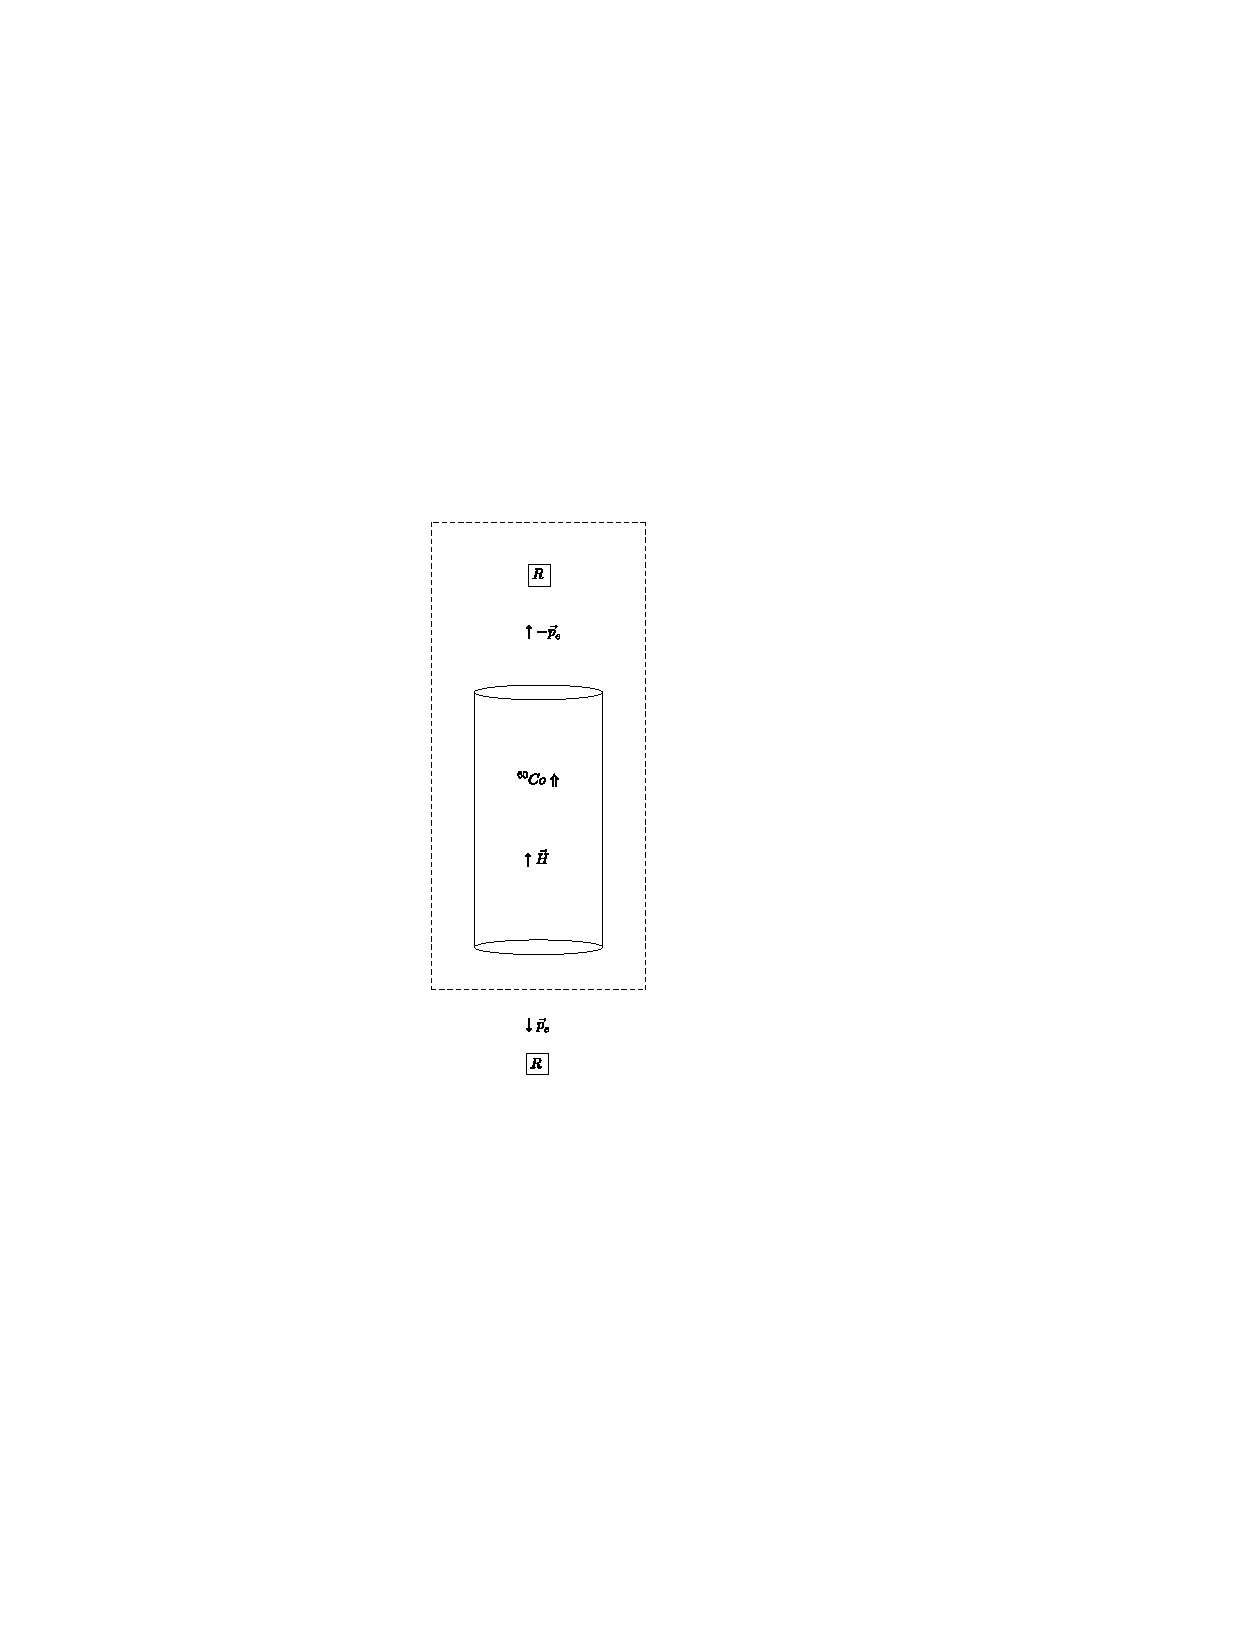
\includegraphics{img/dis_pboh1}
\end{figure}
Gli eventi osservati dall'osservatore di sopra saranno quelli spazialmente
riflessi dagli eventi osservati dall'osservatore di sotto. Questo perchè $p$ 
cambia segno,
mentre $H$ e lo spin no. In questo ragionamento abbiamo assunto che i nuclei di 
$\text{Co}^{60}$ sono a riposo in mdo da essere invarianti per inversione 
spaziale.
Quindi se nel processo fosse rispettata la simmetria per inversione spaziale i 
due rivelatori dovrebbero contare lo stesso numero di elettroni $\beta$ per 
unità di tempo.

Conteggi differenti implicherebbero una violazione della simmetria per 
inversione spaziale. Per effettuare le misure si utilizzò un solo rivelatore 
invertendo il senso della
corrente nel solenoide (vedi \autoref{dis_testo}). L'esperimento rivelò che 
gli elettroni venivano emessi in numero maggiore nella direzione opposta allo 
spin nucleare.
Si trovò che il fascio di elettroni emessi aveva una distribuzione angolare 
del tipo:
\[
I(\theta)=I_0(1-\frac{v}{c}\cos\theta)
\]
dove $\theta$ è l'angolo fra la direzione di emissione e lo spin nucleare.
Se fosse stata mantenuta la simmetria per inversione spaziale la dipendenza 
doveva essere del tipo $\cos^{2n}\theta$, in modo da avere simmetria attorno al 
piano azimutale
(vedi \autoref{dis_testo2}).
\begin{figure}[!hbt]
\centering
\caption{Seconda figura del testo originale.}
\label{dis_testo2}
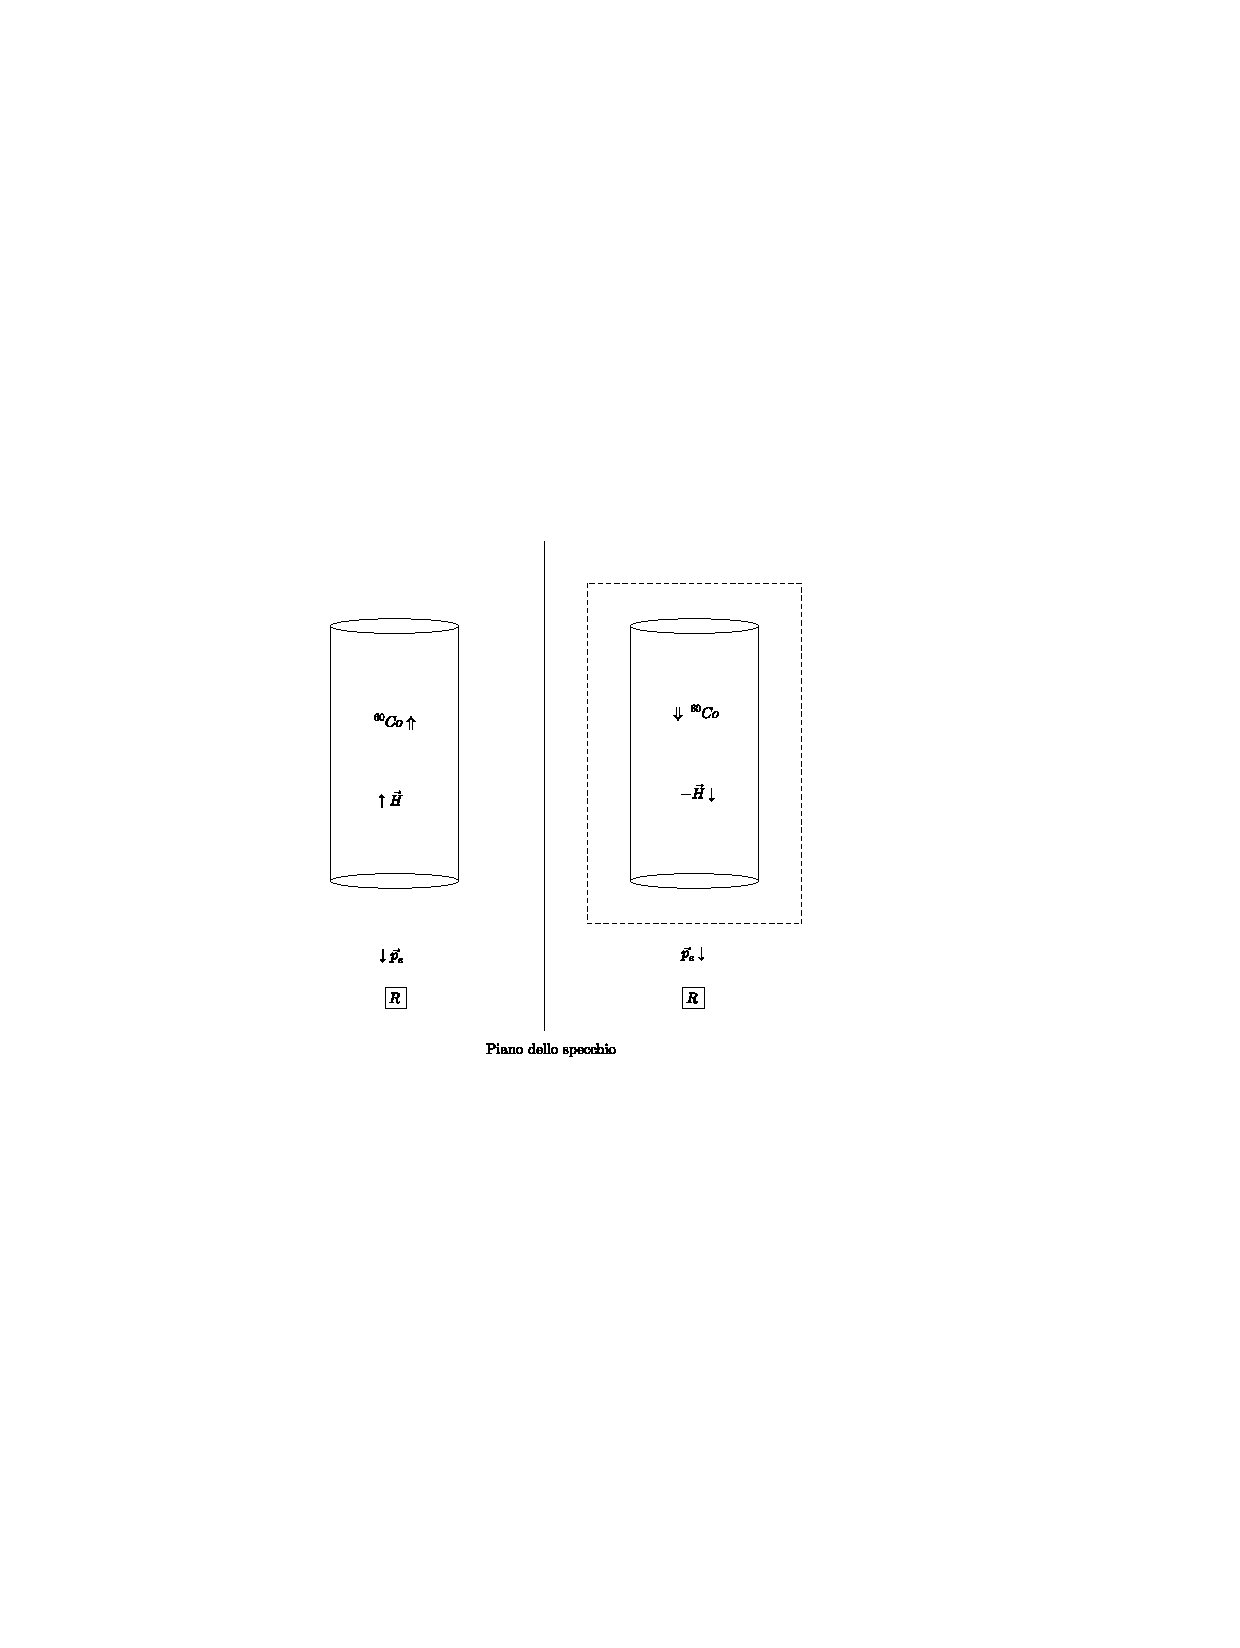
\includegraphics{img/dis_pboh2}
\end{figure}
L'importanza di questo esperimento è proprio la scoperta della violazione del 
principio di invarianza per inversione spaziale. Prima si credeva che il 
risultato di un esperimento
dovesse essere lo stesso se si usa un sistema o quello speculare.

Analizziamo\marginnote{6-3-1998} ora più in dettaglio questo esperimento e 
come è stato ricavato il risultato $\langle 
H\rangle_{e_{\beta}^-}=-\frac{v}{c}$.
Nella reazione
\[
\text{Co}^{60}\rightarrow \text{Ni}^{60}+e^-+\bar{\nu}
\]
lo spin nucleare diminuisce di un'unità pur rimanendo parallelo ad 
$\mathcal{H}$. La coppia elettrone-antineutrino ha momento angolare nullo 
rispetto al nucleo.
Per la conservazione del momento angolare totale l'elettrone e l'antineutrino 
devono avere spin $1/2$, orientato sempre nella stessa direzione:
\[
\Uparrow_{\text{Co}^{60}}\quad\Uparrow_{\text{Ni}^{60}}\quad\Uparrow_{1/2}\quad\
Uparrow_{1/2}
\]
Quindi un elettrone emesso longitudinalmente alla direzione dello spin avrà 
una polarizzazione longitudinale, quindi sarà in un autostato dell'elicità.
Per un angolo di emissione $\theta=0$ l'autovalore dell'elicità è $+1$, per 
$\theta=\pi$ l'autovalore dell'elicità è $-1$.
Indichiamo con $I_+$ e $I_-$ le intensità dei fasci di elettroni con 
$\theta=0$ e $\theta=\pi$. Il valore medio dell'elicità per un singolo 
elettrone sarà:
\[
\frac{(+1)I_++(-1)I_-}{I_++I_-}
\]
Abbiamo già detto che il risultato sperimentale per l'intensità è:
\begin{align*}
&I(\theta)=I_0(1-\frac{v}{c}\cos\theta)\\
&I_+=I(0)=I_0(1-\frac{v}{c})\\
&I_-=I(\pi)=I_0(1+\frac{v}{c})
\end{align*}
Quindi il valore medio di elicità risulta essere:
\[
\frac{(+1)I_+(-1)I_-}{I_++I_-}=-\frac{v}{c}
\]
\begin{itemize}
 \item Inversione spaziale = inversione di tutti e tre gli assi.
 \item Inversione speculare = inversione di un solo asse.
\end{itemize}
Queste due operazioni differiscono solo per una rotazione di $\pi$\footnote{\`E
presente nel testo una riga, purtroppo tagliata nella fotocopia, che risulta
illeggibile. (Ovviamente il professore vi chiederà quella)}.

Il sistema risulta simmetrico per inversione spaziale solo perché i nuclei di 
cobalto sono fermi, se così non fosse non si avrebbe questa simmetria iniziale 
e quindi non
ci si stupirebbe di riscontrare una asimmetria nei risultati.
\chapter{Teoria di Fermi}

Nel 1934 Fermi formulò una teoria fenomenologica del decadimento $\beta$ in 
accordo con i risultati sperimentali. Questo lavoro inaugurò la fisica delle 
particelle nucleari.
Questa teoria non prevedeva la violazione della simmetria speculare, ma lo 
schema di questa teoria rimane valido ancora oggi. Uno dei risultati di questa 
teoria è la spiegazione
degli spettri $\beta$. Sia $N_e$ il numero di elettroni emessi in un certo 
intervallo di tempo con un'energia cinetica compresa fra 
$[0,T_{\text{e,max}}]$, la distribuzione
di energia è data dalla funzione
\[
f(T_e)=\frac{dN_e}{dT_e}=\text{funzione di distribuzione}
\]
dove $dN_e$ è il numero di elettroni emessi con energia cinetica compresa 
nell'intervallo $[T_e,T_e+dT_e]$. Ovviamente deve essere:
\[
N_e=\int_0^{T_{\text{e,max}}}\frac{dN_e}{dT_e}dT_e
\]
Un altro importante risultato è la relazione fra $T_{\text{e,max}}$ e la vita 
media del nucleo che decade. Sulla base di questa teoria si possono enunciare 
alcune regole di selezione
che permettono una classificazione dei diversi decadimenti $\beta$ e la 
spiegazione del perché alcuni decadimenti sono meno favoriti di altri.

Il punto di partenza della teoria è la constatazione che l'interazione che 
determina il decadimento $\beta$ deve essere molto più piccola di quella 
elettromagnetica.

Consideriamo un nucleo a riposo di massa $M$ che decade in un nucleo di massa 
$M'$. Si ha che:
\begin{align*}
&Mc^2=M'c^2+Q\\
&Q=Mc^2-M'c^2=\text{Energia disponibile per la transizione}
\end{align*}
Questo parametro caratterizza la transizione e rappresenta tutta l'energia 
interna che il nucleo iniziale perde. L'energia di decadimento $E_d$ è la sola 
energia cinetica
che si genera nella transizione, infatti per definizione si ha:
\[
E_d=Mc^2-M'c^2-\sum_i m_ic^2
\]
quindi questa non caratterizza il decadimento come $Q$ perché dipende anche 
dalle masse delle altre particelle prodotte. Sperimentalmente si ha che a 
parità di $Q$ un nucleo che decade
per emissione $\beta$ ha vita media molto più lunga di quella di un nucleo che 
decade per emissione $\gamma$ ($Q\simeq1\si{\mega\electronvolt}$, 
$\tau_{\gamma}\simeq10^{-15}\si{\second}$,
$\tau_{\beta}\simeq10\text{min}$).
Questo fatto significa che $\lambda_{\beta}\ll\lambda_{\gamma}$, quindi la 
probabilità di decadimento è più piccola per un decadimento $\beta$ rispetto 
a quello $\gamma$.
Un altro fatto sperimentale è che:
\[
\tau_{\gamma}\gg 
T\equiv\frac{\hbar}{E}\simeq10^{-27}\si{\second}\quad(E\simeq100\,\si{\giga\elec
tronvolt})
\]
dove $T\cdot2\pi$ è il periodo caratteristico di oscillazione della funzione 
d'onda nucleare ($e^{-\frac{i}{\hbar}Et}$). Quindi nell'emissione $\gamma$ 
prima di decadere il nucleo
si trova in uno stato imperturbato il cui livello energetico coincide con il 
livello di energia $E$ a meno del parametro 
$\Gamma=\frac{\hbar}{\tau_{\gamma}}<<E$. Quindi l'intensità
dell'interazione $\beta$ è molto più piccola di quella $\gamma$. Da questo 
nasce il nome di \textit{interazione debole} per l'interazione responsabile del 
decadimento $\beta$.
L'hamiltoniana corrispondente risulterà molto più piccola di quella nucleare. 
Quindi possiamo usare la teoria delle perturbazioni fermandoci al primo ordine.
Sia $\mathcal{H}$ l'hamiltoniana totale del nucleo che decade. Si può scrivere 
nella rappresentazione di Schr\"{o}dinger:
\[
\mathcal{H}=\mathcal{H}_0+\mathcal{H}_{\text{int}}
\]
$\mathcal{H}_{\text{int}}$ non dipende dal tempo in quanto il sistema in esame 
è un sistema chiuso. Se passiamo dalla rappresentazione di interazione invece 
si ha:
\[
\mathcal{H}_I(t)=\mathcal{H}_0+\mathcal{H}_{\text{Iint}}(t)
\]
Lavoreremo sempre in questa rappresentazione, quindi in seguito sarà omesso il 
pedice $I$.

Possiamo assumere che il nucleo si trovi inizialmente nello stato $|i\rangle$, 
che sia autostato di $\mathcal{H}_0$ con autovalore $E_i$. Questa assunzione è 
esatta solo se l'istante iniziale
è $t=-\infty$, nella realtà non è così, ma dato che il nucleo ha una vita 
estremamente lunga questa è una buona approssimazione. Indichiamo con 
$|t\rangle$ lo stato del sistema
all'istante $t$. Si può scrivere:
\[
i\hbar\frac{d}{dt}|t\rangle=\mathcal{H}_{\text{int}}(t)|t\rangle
\]
con la condizione iniziale
\[
|t=0\rangle=|i\rangle
\]
Supponiamo \marginnote{9-3-1998} che i possibili stati finali abbiano uno 
spettro discreto. Questi stati finali sono autostati di $\mathcal{H}_0$. Si 
può scrivere:
\[
|t\rangle=\sum_fc_f(t)|f\rangle=\sum_{f\neq i}c_f(t)|f\rangle+c_{f= 
i}|f=i\rangle
\]
dove i coefficienti $c_f(t)$ sono definiti come:
\[
c_f(t)=\langle f|t\rangle
\]
Il modulo quadro di $c_f(t)$ dà la probabilità che all'istante $t$ il sistema 
si trovi nello stato $f$. Per la condizione iniziale deve essere:
\[
|c_{f\neq i}(0)|^2=0\quad |c_{f=i}|^2=1
\]
Per questo motivo le quantità $|c_f|^2(f\neq i)$ si dicono 
\textit{probabilità di transizione}. Lo stato finale può non avere energia 
uguale a quella iniziale.
Questo perché l'energia del sistema fra $t=0$ e $t$ è soggetta alla relazione:
\[
\Delta E_i=\frac{\hbar}{t}
\]
Quindi le transizioni possono avvenire fra stati la cui energia è compresa 
nell'intervallo $[E_i-\frac{\Delta E_i}{2},E_i+\frac{\Delta E_i}{2}]$.
Deve però essere sempre verificato che:
\[
\langle\mathcal{H}\rangle=\langle t|\mathcal{H}(t)|t\rangle=E_i
\]
La quantità $\frac{\Delta E_i}{2}$ non può superare il valore di $E_i$, 
quindi:
\[
\Delta E_i\leq2E_i
\]
Le probabilità di transizione risulteranno molto minori di $1$, quando la 
pertirbazione $\mathcal{H}_{\text{int}}(t)$ è molto piccola, anche per $t$ 
molto grandi, cioé:
\[
|C_{f\neq i}|^2<<1\quad(t>>\frac{\hbar}{E_i})
\]
Ma in queste condizioni (essendo $t=\frac{\hbar}{\Delta E_i}$) deve essere 
$\Delta E_i<<E_i$. Avvengono quindi transizioni a stati finali la cui energia 
è $E_f\simeq E_i$.
La condizione $E_f=E_i$ è esatta se $\mathcal{H}_{\text{int}}$ è un 
infinitesimo. Infatti in questo caso una transizione  ad uno stato può 
avvenire solo per $t$ tendente ad infinito:
\[
\lim_{t\rightarrow+\infty}\Delta E_i=\lim_{t\rightarrow+\infty}\frac{\hbar}{t}=0
\]
Possiamo assumere per l'hamiltoniana di interazione $\beta$ che questa sia un 
infinitesimo rispetto ad $\mathcal{H}_0$, e quindi la transizione può avvenire 
solo a $t\rightarrow+\infty$.
In queste ipotesi si hanno transizioni fra stati che hanno energia finale 
uguale a quella iniziale.

Passiamo ora ad una trattazione più rigorosa considerando tutti i possibili 
stati finali. Per un lungo intervallo a partire da $t=0$ si ha:
\[
|c_{f\neq i}(t)|^2\simeq |c_{f\neq i}(0)|^2=0
\]
Se ci si ferma al primo ordine nella teoria delle perturbazioni si può 
scrivere:
\[
|c_{f\neq 
i}(t)|^2=2|\mathcal{H}_{\text{if}}|^2\frac{1-\cos(\omega_{\text{if}}t)}{(E_f-E_i
)^2}
\]
dove si è posto:
\begin{align*}
&\omega_{\text{if}}=\frac{E_f-E_i}{\hbar}\\
&|\mathcal{H}_{\text{if}}|^2\equiv\langle 
f|\mathcal{H}_{\text{int}}|i\rangle\propto e^{i\omega_{\text{if}}t}\quad 
(|f\rangle\neq|i\rangle)\\
&|\mathcal{H}_{\text{if}}|^2=\text{costante}
\end{align*}
(questo si può dedurre considerando che i prodotti scalari non dipendono dalla 
rappresentazione).
\[
\frac{d}{dt}|c_{f\neq 
i}(t)|^2=\frac{2}{\hbar}|\mathcal{H}_{\text{if}}|^2\frac{\sin(\omega_{\text{if}}
t)}{E_f-E_i}
\]
Attenzione!\footnote{Nel testo è presente, scritta minuscola, la formula
  $\frac{d}{dt}|c_{f\neq
  
i}|^2=2|\mathcal{H}_{\text{if}}|^2\,\frac{\sin(\omega_{\text{if}}t)}{(E_f-E_i)^2
}\omega_{\text{if}}$.
Questa è la stessa formula a meno delle semplificazioni.}

Se approssimiamo $\mathcal{H}_{\text{int}}$ ad un infinitesimo, 
$\mathcal{H}_{\text{if}}$ lo sarà pure.
In questo caso dobbiamo considerare il limite:
\begin{align*}
&\lim_{t\rightarrow+\infty}\bigl[\frac{d}{dt}|c_{f\neq 
i}(t)|^2\bigr]=\frac{2}{\hbar}|\mathcal{H}_{\text{if}}|^2\lim_{t\rightarrow+\inf
ty}\frac{\sin(\omega_{\text{if}}t)}{E_f-E_i}\\
&\lim_{t\rightarrow+\infty}\frac{\sin(\omega_{\text{if}}t)}{E_f-E_i}=\frac{\pi}{
\hbar}\lim_{t\rightarrow+\infty}\frac{\sin(\omega_{\text{if}}t)}{\pi\omega_{\tex
t{if}}}=\frac{\pi}{\hbar}\delta(\omega_{\text{if}})\\
&\delta(\omega_{\text{if}})=\lim_{t\rightarrow+\infty}\frac{\sin(\omega_{\text{i
f}}t)}{\pi\omega_{\text{if}}}=\hbar\lim_{\frac{t}{\hbar}\rightarrow+\infty}\frac
{\sin[(E_f-E_i)t/\hbar]}{\pi(E_f-E_i)}=\hbar\delta(E_f-E_i)
\end{align*}
L'uguaglianza fra la funzione $\delta$ ed il limite è un'uguaglianza fra 
funzionali e non fra funzioni.
Quindi\marginnote{11-3-1998} nel limiti di un'hamiltoniana di interazione 
infinitesima saranno accessibili solo stati finali con $E_f=E_i$.
\[
W_{\text{if}}=\lim_{t\rightarrow+\infty}[\frac{d}{dt}|c_{f\neq 
i}(t)|^2]=\frac{2\pi}{\hbar}|\mathcal{H}_{\text{if}}|^2\delta(E_f-E_i)=\text{cos
tante}
\]
Questa è la probablità di transizione  da $i$ ad $f$ nell'unità di tempo. Si 
può definire la probabilità totale di transizione nell'unità di tempo come:
\[
W=\sum_{f\neq i}W_{\text{if}}=\frac{2\pi}{\hbar}\sum_{f\neq 
i}|\mathcal{H}_{\text{if}}|^2\delta(E_f-E_i)=\text{Probabilità totle di 
transizione nell'unità di tempo.}
\]
Di fatto si ha che $W_{\text{if}}=0$ se $E_f\neq E_i$, quindi gli unici 
contributi provengono da stati $f$ con $E_f=E_i$.

Tutti i risultati sono stati trovati lavorando al primo ordine. Se consideriamo 
anche ordini sccessivi di approssimazione allora il procedimento al limite 
porta sempre ad una $W$ costante.
Quindi si può scrivere la probabilità totale mediante la formula:
\[
W=\frac{2\pi}{\hbar}\sum_{f\neq i}|T_{\text{if}}|^2\delta(E_f-E_i)
\]
dove $T_{\text{if}}$ ha le dimensioni di energia. Questi coefficienti si dicono 
elementi di matrice relativi alla transizione dallo stato $i$ allo stato $f$.

Fino ad ora abbiamo lavorato sull'ipotesi di spettro discreto. Di solito si 
hanno spettri continui, sappiamo che questi però possono essere approssimati 
con spettri quasi continui.
Per fare questa approssmazione si deve introdurre la densità di stati finali 
come:
\[
\rho_f(E_f)=\frac{dN}{dE_f}|_{E_f}\quad\text{$dN=$ numero di stati finali con 
energia compresa nell'intervallo $[E_f,E_f+dE_f]$.}
\]
E si deve fare la sostituzione:
\[
\sum_f\rightarrow\int N=\int\rho_f(E_f)dE_f
\]
Quindi la probabilità totale nell'unità di tempo $W$ diventa:
\[
W=\frac{2\pi}{\hbar}\int|\mathcal{H}_{\text{if}}|^2\delta(E_i-E_f)\rho_f(E_f)dE_
f=\frac{2\pi}{\hbar}|T_{\text{if}}|^2\rho_f(E_i)
\]
dove in prima approssimazione si può scrivere:
\[
W=\frac{2\pi}{\hbar}|\mathcal{H}_{\text{if}}|^2\rho_f(E_i)\quad\text{\textsc{Reg
ola d'oro
di Fermi}}
\]
Secondo questa formula $W$ è data dal prodotto di due fattori: uno di natura 
dinamica ($|\mathcal{H}_{\text{if}}|^2$), mentre l'altro è non dinamico ed è 
la densità
di stati finali con $E_f=E_i$: $\rho_f(E_i)=\frac{dN}{dE_f}|_{E_f=E_i}$.

Se si vuole passare al caso continuo dal caso quasi continuo si deve fare il 
limite per $V\rightarrow+\infty$ dove $V$ è il volume della scatola.

Se vogliamo applicare la regola d'oro al decadimento $\beta^-$ si deve 
specificare l'elemento di matrice $T_{\text{if}}$, che al primo ordine è 
$\mathcal{H}_{\text{if}}$.
L'hamiltoniana di interazione rappresenta una perturbazione piccola in 
confronto all'hamiltoniana nucleare, quindi:
\[
\tau_{\beta}>>\tau_{\gamma}>>T=\frac{\hbar}{E}
\]
Si può quindi assumere $\tau_{beta}=\infty$. Nell'intervallo di tempo fra $0$ 
e $\tau_{\beta}$ la funzione d'onda quasi stazionaria si può scrivere come:
\[
\begin{split}
\psi 
&=\psi(0)e^{-\frac{i}{\hbar}Et}e^{-\frac{t}{2\tau_{\beta}}}=\psi(0)e^{-i\frac{t}
{T}-\frac{t}{2\tau_{\beta}}}\simeq\\
&\simeq\psi(0)e^{-i\frac{t}{T}}=\psi(0)e^{-\frac{i}{\hbar}Et}\quad(0\leq 
t<\tau_{\beta})\quad(\text{Questo è uno stato stazionario.})
\end{split}
\]
Quindi in questa approssimazione il nucleo si trova in uno stato non perturbato 
per tutto il tempo di vita media. Per questo il decadimento $\beta$ si può 
considerare
come un processo dinamico di durata istantanea. Secondo la teoria della 
relatività tutte le interazioni hanno una velocità di propagazione finita. 
Quindi il decadimento $\beta$
può avvenire solo in una regione puntiforme del nucleo (la sua durata è 
istantanea).
Per questo il decadimento $\beta$ coinvolge un solo nucleone ed è lecito 
scrivere:
\[
n\rightarrow p^++e^-+\bar{\nu}
\]
Quindi $\mathcal{H}_{\text{int}}$ di un nucleo soggetto ad un decadimento 
$\beta^-$ è identica a quella di un neutrone che decade in un protone.
\breaknote

In\marginnote{13-3-1998} base alla teoria di Dirac un fermione con 
quadriimpulso $p^{\mu}$ che viene creato in un punto spaziotemporale è 
equivalente alla distruzione di
un fermione con quadrimpulso opposto nello stesso punto spaziotemporale. Quindi 
se a $\bar{\nu}$ che viene creato sostituiamo un $\nu$ distrutto possiamo 
considerare
il processo di diffusione:
\[
n+\nu\rightarrow p^++e^-\quad(\Leftrightarrow n\rightarrow p^++e^-+\bar{\nu} 
\text{ decadimento $\beta^-$})
\]
che è caratterizzato dalla stessa $\mathcal{H}_{\text{int}}$ del processo di 
sopra. Il decadmento $\beta^-$ di un neutrone equivale dal punto di vista 
dinamico al processo rappresentato nel
diagramma in \autoref{fig:dia_fey}.
\begin{wrapfigure}{l}{5.5cm}
\centering
\caption{}
\label{fig:dia_fey}
\begin{tikzpicture}[scale=1, >=triangle 45]
  \draw [->] (-2,-2) -- (-1,-1) node [right=10pt] {$n$};
  \draw [->] (-1,-1) -- (1,1) node [right=10pt] {$e^-$};
  \draw (1,1) -- (2,2);
  \draw [->] (2,-2) -- (1,-1) node [right=10pt] {$\nu$};
  \draw [->] (1,-1) -- (-1,1) node [left=10pt] {$p^+$};
  \draw (-1,1) -- (-2,2);
  \filldraw (0,0) circle (1pt);
  \begin{scope}[>=stealth]
    \draw [<-] (.2,0) -- (2,0) node [right=5pt] {vertice};
  \end{scope}
\end{tikzpicture}
\end{wrapfigure}

In questo processo sono coinvolte quattro particelle (due entranti e due 
uscenti). Queste interagiscono solo nel punto di incontro che si dice 
\textit{vertice del diagramma}.
Un'interazione caratterizzata da un solo vertice si dice \textit{interazione di 
contatto} oppure \textit{processo del primo ordine}.

In un processo di diffusione di due particelle  il potenziale di interazione 
dipenderà solo da $|\vec{r_1}-\vec{r_2}|$. Supponiamo che le due particelle 
siano descritte da funzioni d'onda
scalari, siano queste $\psi_1(\vec{r_1})$, $\psi_2(\vec{r_2})$. Per definizione 
si ha:
\[
\mathcal{H}_{\text{if}}=\langle f|\mathcal{H}_{\text{int}}|i\rangle=\int 
\psi^*_{1f}(\vec{r_1})\psi^*_{2f}(\vec{r_2})V(|\vec{r_1}-\vec{r_2}|)\psi_{1i}(\v
ec{r_1})\psi_{2i}(\vec{r_2})d^3r_1d^3r_2
\]
Questa formula vale anche per una diffusione anelastica, cioé anche se le 
particelle subiscono trasformazioni interne. Nel caso che stiamo considerando 
si ha un \textit{potenziale di contatto},
quindi il potenziale si può scrivere come:
\[
V(|\vec{r_1}-\vec{r_2}|)=g\delta^3(|\vec{r_1}-\vec{r_2}|)
\]
dove $g$ è una costante da determinare sperimentalmente. Con questa scelta per 
$V$ possiamo calcolare l'elemento di matrice:
\[
\mathcal{H}_{\text{if}}=g\int 
\psi^*_{1f}(\vec{r})\psi^*_{2f}(\vec{r})\psi_{1i}(\vec{r})\psi_{2i}(\vec{r})d^3\
vec{r}
\]
Questa in realtà non è esatta in quanto le particelle hanno uno spin $1/2$ e 
quindi le funzioni d'onda non sono scalari ma spinori. Per il momento comunque 
trascureremo questo fatto. Poniamo:
\[
\psi_{1i}=\psi_n;\quad\psi_{2i}=\psi_{\nu};\quad\psi_{1f}=\psi_p;\quad\psi_{2f}=
\psi_e
\]
Si ottiene dunque (V = volume nucleare):
\[
\mathcal{H}_{\text{if}}^{(\beta)}=g\int_V\psi^*_p(\vec{r})\psi^*_e(\vec{r})\psi_
n(\vec{r})\psi_{\nu}(\vec{r})d^3\vec{r}
\]
questo integrale è esteso al volume nucleare e $\vec{r}$ rappresenta la 
posizione del neutrone rispetto al centro del nucleo. La costante $g$ si dice 
\textit{costante di accoppiamento di Fermi}.
Questa ha le dimensioni di energia per volume. Le due funzioni d'onda 
$\psi^*_e$ e $\psi_{\nu}$ si possono scrivere nella forma stazionaria:
\begin{align*}
&\psi_e^*(\vec{r})=\frac{1}{\Omega^{1/2}}e^{-i\vec{k_e}\cdot\vec{r}}\\
&\psi_{\nu}(\vec{r})=\frac{1}{\Omega^{1/2}}e^{i\vec{k_{\nu}}\cdot\vec{r}}
\end{align*}
con
\begin{align*}
&\vec{k_e}=\frac{1}{\hbar}\vec{p}\\
&\vec{k}_{\nu}=-\vec{k}_{\bar{\nu}}
\end{align*}
$\Omega$ è il volume dove è racchiuso il sistema\footnote{Quello relativo 
all'approssimazione al caso quasi continuo. .}.
Con questa scelta si trascurano le interazioni tra il neutrino o l'elettrone 
con il nucleo\footnote{Ad esempio si trascurano le forze elettromagnetiche. }.
Di solito gli impulsi di $e^-$ e $\nu$ sono di un ordine di grandezza tale che:
\[
  
\text{\textcrlambda}=\frac{\lambda}{2\pi}=\frac{1}{k}=\frac{\hbar}{p}\gtrsim2\cd
ot10^{-11}\,\si{\centi\meter}
\]
Quindi \textcrlambda è molto grande in confronto alle dmensioni nucleari. Se 
poniamo:
\begin{align*}
&e^{-i\vec{k_e}\cdot\vec{r}}=1-i\vec{k_e}\cdot\vec{r}+\dots\\
&e^{i\vec{k_{\nu}}\cdot\vec{r}}=1+i\vec{k_{\nu}}\cdot\vec{r}+\dots
\end{align*}
si avrà che per ogni punto $\vec{r}$ interno al nucleo:
\[
\vec{k_e}\cdot\vec{r}<<1;\quad\vec{k_{\nu}}\cdot\vec{r}<<1
\]
Ci si può dunque fermare ai termini di ordine zero nello sviluppo in serie:
\[
\psi_e^*(\vec{r})\psi_{\nu}(\vec{r})\simeq\psi_e^*(0)\psi_{\nu}(0)=\frac{1}{\Ome
ga}
\]
questa approssimazione è possibile a patto che l'elemento di matrice che si 
ottiene non risulti nullo. Ogni volta che questo è verificato si può scrivere:
\begin{align*}
&\mathcal{H}_{\text{if}}^{(\beta)}\simeq 
g\int\psi_p^*(\vec{r})\psi_n(\vec{r})\psi_e^*(0)\psi_{\nu}(0)d^3\vec{r}\neq0\\
&\mathcal{H}_{\text{if}}^{(\beta)}\simeq\mathcal{H}_{\text{if}}^{(0)}\equiv 
g\frac{M_{\text{if}}}{\Omega}\,\text{dove}\quad 
M_{\text{if}}=\int\psi_p^*(\vec{r})\psi_n(\vec{r})d^3\vec{r}
\end{align*}
dove $M_{\text{if}}$ è un numero puro. Questa approssimazione corrisponde 
all'approssimazione di monopolo, e il nucleo non è altro che un punto rispetto 
a $\lambda_e$ e $\lambda_{\nu}$.
Quindi l'elettrone e l'antineutrino non possono avere un $L$ rispetto al nucleo
in quanto sono stati emessi da una sorgente puntiforme. Quindi il sistema 
$e^-+\bar{\nu}$ ha due possibilità
per il momnto angolare totale: $0$ (singoletto), $1$ (tripletto). Nel primo caso
si parla di \textit{transizione di Fermi}, nel secondo caso si dice 
\textit{transizione di Gamow Teller}.
Nel primo caso vale la regola di selezione di Fermi secondo cui le transizioni 
permesse sono solo quelle per cui:
\[
  \Delta j=j_f-j_i=0\quad\text{\textsc{Regola di Fermi}}
\]
Nel secondo caso vale la regola di selezione di Gamow-Teller secondo cui è
proibita ogni transizione con \#\#\#\footnote{Cosa stranissima: lo spazio è
bianco anche nel testo, ed è presente una freccina
con un punto interrogativo? Era finito l'inchiostro? Sbobinatura non chiara?
Prossimamente a Voyager! NdT.}, mentre sono permesse solo transizioni per cui:
\[
 j_{\text{fin}}-1\leq j_{\text{in}}\leq j_{\text{fin}}+1
\]
che implica
\[
\begin{sistema}
\Delta j=\pm1\\
\Delta j=0\;(i\neq0)
\end{sistema}\qquad\text{\textsc{Regola di selezione di Gamow-Teller}}
\]
In particolare la transizione $\beta$ del $\text{Co}^{60}$ è una transizione di
Gamow-Teller ``permessa''. Queste regole di selezione valgono solo nelle 
approssimazioni considerate
perché sono state dedotte dall'ipotesi che fosse nullo il momento orbitale del
sistema $e^-+\bar{\nu}$. Nella risoluzione esatta del problema si trovano delle 
transizioni $\beta$ che
non rientrano fra le regole di selezione enunciate, queste transizioni però 
sono
meno favorite in quanto i corrispondenti elementi di matrice sono di ordine più
piccolo rispetto
agli elementi di matrice della transizione permessa.

Abbiamo\marginnote{16-3-1998} visto che sotto certe ipotesi si ha: 
$\mathcal{H}_{\text{if}}=g\frac{M_{\text{if}}}{\Omega}$.
Abbiamo anche ricavato le regole di selezione e commentato la loro validità. Se
consideriamo solo le transizioni permesse, la regola d'oro di Fermi assume la
forma:
\[
W=\frac{2\pi}{\hbar}|\mathcal{H}_{\text{if}}(0)|^2\rho_f(E_i)=\frac{2\pi}{\hbar\
Omega^2}g^2|M_{\text{if}}|^2\rho_f(E_i)
\]
L'elemento di matrice $\mathcal{H}_{\text{if}}$ che compare in $W$ non dipende
dai momenti delle particelle interagenti, quindi questa può essere interpretata
come probabilità di transizione
complessiva nell'unità di tempo per tutti i possibili valori dei momenti. 
Questa
interpretazione è corretta se $\rho_f(E_i)$ è la densità complessiva di stati
finali con energia $E_i$.
Quindi $W$ è la probabilità di decadimento $\beta$ nell'unità di tempo, 
dunque deve essere:
\[
W=\lambda_{\beta}
\]
Se poniamo per l'energia finale $E_f$:
\[
E_f=M'c^2+Q
\]
dove $M'$ è la massa del nucleo prodotto e $Q$ l'energia disponibile. Si avrà:
\[
dE_f=dQ\Rightarrow\rho_f=\frac{dN}{dE_f}|_{E_f=E_i}=\frac{dN}{dQ}|_{Q=E_i-M'c^2}
\]
dove $dN$ è il numero totale di stati finali con energia compresa fra $E_i$ e
$E_i+dQ$. Per l'energia $Q$ si avrà:
\[
Q=E_e+E_{\bar{\nu}}+T_R
\]
dove $E_e$ è l'enrgia totale dell'elettrone, $E_{\bar{\nu}}$ l'energia totale
dell'antineutrino, $T_R$ l'energia di rinculo del nucleo.
Ma dal momento che $T_R<<E_e,E_{\bar{\nu}}$ si ha:
\[
Q=E_e+E_{\bar{\nu}}=(m_e^2c^4+c^2p_e^2)^{1/2}+cp_{\bar{\nu}}
\]
La forma dello spettro\footnote{Spettro $\beta=$ numero di elettroni con una
certa energia} $\beta$ si può ricavare direttamente dalla conoscenza della
funzione:
\[
\frac{dW}{dE_e}=\frac{dW}{dT_e}
\]
Il numero $M_{\text{if}}$ non dipende da $T_e$, allora la forma dello spettro
$\beta$ è determinata solo dalla conoscenza della funzione $\rho_f(E_i)$.
Dobbiamo calcolare la funzione:
\[
\frac{d\rho_f}{dT_e}=\frac{d^2N}{dT_edQ}
\]
in quanto:
\[
\frac{dW}{dT_e}\propto\frac{d\rho_f}{dT_e}
\]
Possiamo equivalentemente calcolare la funzione :
\[
\frac{d\rho_f}{dp_e}=\frac{d^2N}{dp_edQ}\quad\text{in 
quanto}\quad\frac{dW}{dp_e}\propto\frac{d\rho_f}{dp_e}
\]
Facciamo l'ipotesi che la scatola immaginaria in cui si suppone racchiuso il 
sistema sia un cubo di lato $L$ con gli spigoli paralleli agli assi $x,y,z$. Si 
potrebbe assumere che le
funzioni d'onda di $e$ e $\bar{\nu}$ si annullino sulle pareti della scatola, 
ma questo non può essere verificato in quanto sono funzioni complesse. La 
condizione meno restrittiva che si può
imporre è che le funzioni d'onda siano invarianti per traslazioni:
\[
x\rightarrow x+L\quad y\rightarrow y+L\quad z\rightarrow z+L
\]
quindi i vettori d'onda devono verificare la condizione:
\[
k_{\alpha}L=2\pi n_{\alpha}\quad(\alpha=x,y,z\;\;n_{\alpha}=0,\pm1,\pm2,\dots)
\]
Lo spettro continuo di $p_e$ e $p_{\bar{\nu}}$ si riduce in questo caso ad uno 
spettro discreto, dove i possibili valori per le componenti sono:
\[
p_{\alpha}=\hbar k_{\alpha}=\frac{2\pi\hbar}{L}n_{\alpha}\quad(\alpha=x,y,z)
\]
Quindi per un dato intervallo $\Delta p_{\alpha}=p_{\alpha}''-p_{\alpha}'>0$ il 
numero di valori che $p_{\alpha}$ può assumere in questo intervallo è:
\[
\Delta n_{\alpha}=n_{\alpha}''-n_{\alpha}'\Rightarrow\frac{\Delta 
n_{\alpha}}{\Delta p_{\alpha}}=\frac{L}{2\pi\hbar}=\text{costante}
\]
Questo rapporto coincide con il numero di autostati di $p_{\alpha}$ per 
intervallo unitario di $p_{\alpha}$. Per ciascuna particella emessa nel 
decadimento la densità di stati è data
dalla quantità:
\[
\frac{\Delta n_x}{\Delta p_x}\frac{\Delta n_y}{\Delta p_y}\frac{\Delta 
n_z}{\Delta 
p_z}=\frac{L^3}{(2\pi\hbar)^3}=\frac{\Omega}{(2\pi\hbar)^3}=\text{densità 
degli stati}
\]
Nell'approssimazione quasi continua il numero di stati di una particella in un 
volumetto $dp_xdp_ydp_z$ è:
\[
\frac{\Omega}{(2\pi\hbar)^3}dp_xdp_ydp_z=\frac{\Omega}{(2\pi\hbar)^3}p^2\sin\the
ta dpd\theta d\phi\quad\text{(in coordinate polari nello spazio dei momenti)}
\]
Il corrispondente numero di stati nell'intervallo $[p,p+dp]$ si ottiene 
integrando su $\theta$ e $\phi$. Per l'elettrone si ottiene:
\[
dN_e=\frac{4\pi\Omega}{(2\pi\hbar)^3}p_e^2dp_e
\]
Per l'antineutrino si ottiene:
\[
dN_{\bar{\nu}}=\frac{4\pi\Omega}{(2\pi\hbar)^3}p^2_{\bar{\nu}}dp_{\bar{\nu}}
\]
Trattandosi di una disintegrazione a tre corpi $p_e$ e $p_{\bar{\nu}}$ possono 
considerarsi indipendenti una dall'altra. Quindi il numero totale di stati 
finali in cui l'elettrone ha la quantità
di moto compresa nell'intervallo $[p_e,p_e+dp_e]$ e l'antineutrino 
nell'intervallo $[p_{\bar{\nu}},p_{\bar{\nu}}+dp_{\bar{\nu}}]$ è:
\[
d^2N=dN_edN_{\bar{\nu}}=\frac{16\pi^2\Omega^2}{(2\pi\hbar)^6}p_e^2dp_ep_{\bar{\n
u}}^2dp_{\bar{\nu}}
\]
Considerato che:
\[
p_{\bar{\nu}}=\frac{Q-E_e}{c}\Rightarrow dp_{\bar{\nu}}=\frac{dQ}{c}
\]
In quanto per calcolare $dp_{\bar{\nu}}$ si deve tenere fisso $dp_e$. 
Sostituendo quest'espressione in quella per $dN^2$ si ottiene:
\begin{align*}
&d^2N=\frac{16\pi^2\Omega^2}{(2\pi\hbar)^6c^3}(Q-E_e)^2p_e^2dp_edQ\\
&\frac{d\rho_f}{dp_e}=\frac{d^2N}{dp_edQ}=\frac{16\pi^2\Omega^2}{(2\pi\hbar)^6c^
3}(Q-E_e)^2p_e^2\\
&\frac{dW}{dp_e}=\frac{2\pi}{\hbar}g^2|M_{\text{if}}|^2\frac{16\pi^2}{(2\pi\hbar
)^6c^3}(Q-E_e)^2p_e^2
\end{align*}
Come ci si doveva aspettare, in questa espressione non compare più il volume 
$\Omega$. Lo spettro $\beta$ così ottenuto rimane valido anche quando $\Omega$ 
è variabile
e quindi anche per $\Omega\rightarrow\infty$. La forma dello spettro $\beta$ 
che si ottiene è rappresentata in \autoref{fig:spettro_beta}.
\begin{figure}[!h]
  \centering
  \caption{Spettro $\beta$.}
  \label{fig:spettro_beta}
  \begin{tikzpicture}[line cap=round,line join=round,>=stealth,x=6.56433537135226cm,y=14.487115647952196cm]
  \draw[->,color=black] (-0.01,0) -- (1.36,0) node [below]
  {$p_e$};
  \foreach \x in {0,0.2,0.4,0.6,0.8,1,1.2}
  \draw[shift={(\x,0)},color=black] (0pt,2pt) -- (0pt,-2pt);
  \draw[->,color=black] (0,-0.01) -- (0,0.33) node [left] {$\frac{\text{d}W}{\text{d}p_e}$};
  \foreach \y in {0,0.1,0.2,0.3}
  \draw[shift={(0,\y)},color=black] (2pt,0pt) -- (-2pt,0pt);
  \clip(-0.01,-0.01) rectangle (1.48,0.35);
  \draw[smooth,samples=100,domain=0:1.35]
  plot(\x,{(\x)^2*sqrt(1.25^2+0.5^2)-(\x)^2*sqrt((\x)^2+0.5^2)});
  \fill [color=\MinorColor] (1.25,0) circle (1.5pt) node [above right]
  {$p_{e,\text{max}}$};
\end{tikzpicture}

\end{figure}
Dalla conoscenza della funzione $\frac{dW}{dp_e}$ si può ricavare il parametro 
$\lambda_{\beta}$, infatti:
\[
\lambda_{\beta}=W=\int_0^{P_{\text{e,max}}}\frac{dW}{dp_e}dp_e
\]
dove
\[
p_{\text{e,max}}=\frac{1}{c}\sqrt{E_{\text{e,max}}^2-m_e^2c^4}\quad\text{con}\;E
_{\text{e,max}}=Q
\]
quindi per $\lambda_{\beta}$ si ottiene:
\[
\lambda_{\beta}=\lambda_{\beta}(p_{\text{e,max}})=\frac{g^2|M_{\text{if}}|^2}{2\
pi^3c^3\hbar^7}\int_0^{p_{\text{e,max}}}[Q-(m_e^2c^4+c^2p_e^2)^{1/2}]^2p_e^2dp_e
\]
Questa espressione ci dà il legame fra $\lambda_{\beta}$ e $p_{\text{e,max}}$, 
o l'energia massima che l'eletrone può avere. Queste formule, con opportune 
correzioni di tipo
elettromagnetico, forniscono valori teorici molto vicini a quelli sperimentali 
per molte transizioni $\beta$ permesse, se però si pone:
\[
g=1,4\cdot10^{-49}\;\text{erg}\cdot\si{\centi\meter}^3\quad 
g\equiv\text{costante di accoppiamento di Fermi.}
\]
